    \chapter{Methodology}



              
        \section{Project requirements(Hardware and software)}
        \subsection{Software Development Model}
 The Agile model is an adaptable and iterative software development process that puts the needs of the client and flexibility first. It breaks the project up into manageable chunks known as sprints or iterations, enabling regular review and modification. Close collaboration between cross-functional teams results in functional software at the conclusion of each iteration. This cycle of iteration guarantees prompt reaction to evolving needs, promoting ongoing enhancement and contentment for the client. The Agile Manifesto's concepts of agile development include a strong emphasis on people and their relationships, functional software, customer collaboration, and adapting to change. In dynamic development contexts, the Agile approach has gained widespread adoption as a framework that encourages efficiency and reactivity.
 \begin{figure}[h]
	\centering
	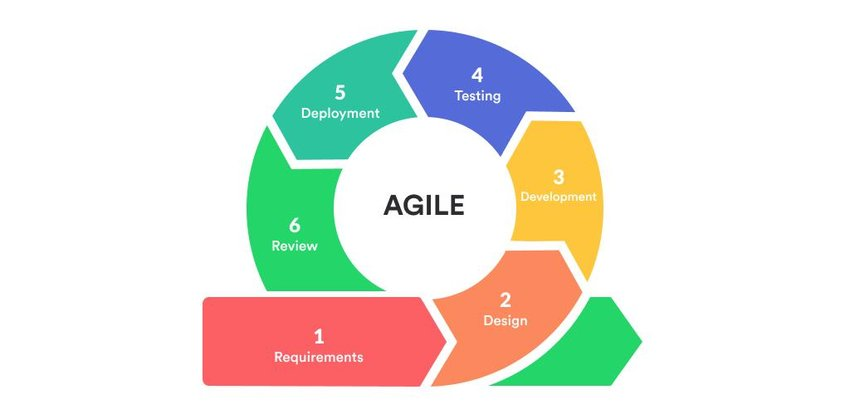
\includegraphics[scale=0.6]{img/Agile_model.png}
	\caption{Agile Model Image.\\   %(Chathmini, 2024). Retrieved from https://medium.com/@chathmini96/agile-methodology-30ec4cdf3fc
}
 
	\end{figure}
	
\pagebreak

\section{Block Diagram}	
	
\begin{figure}[h]
    \centering
    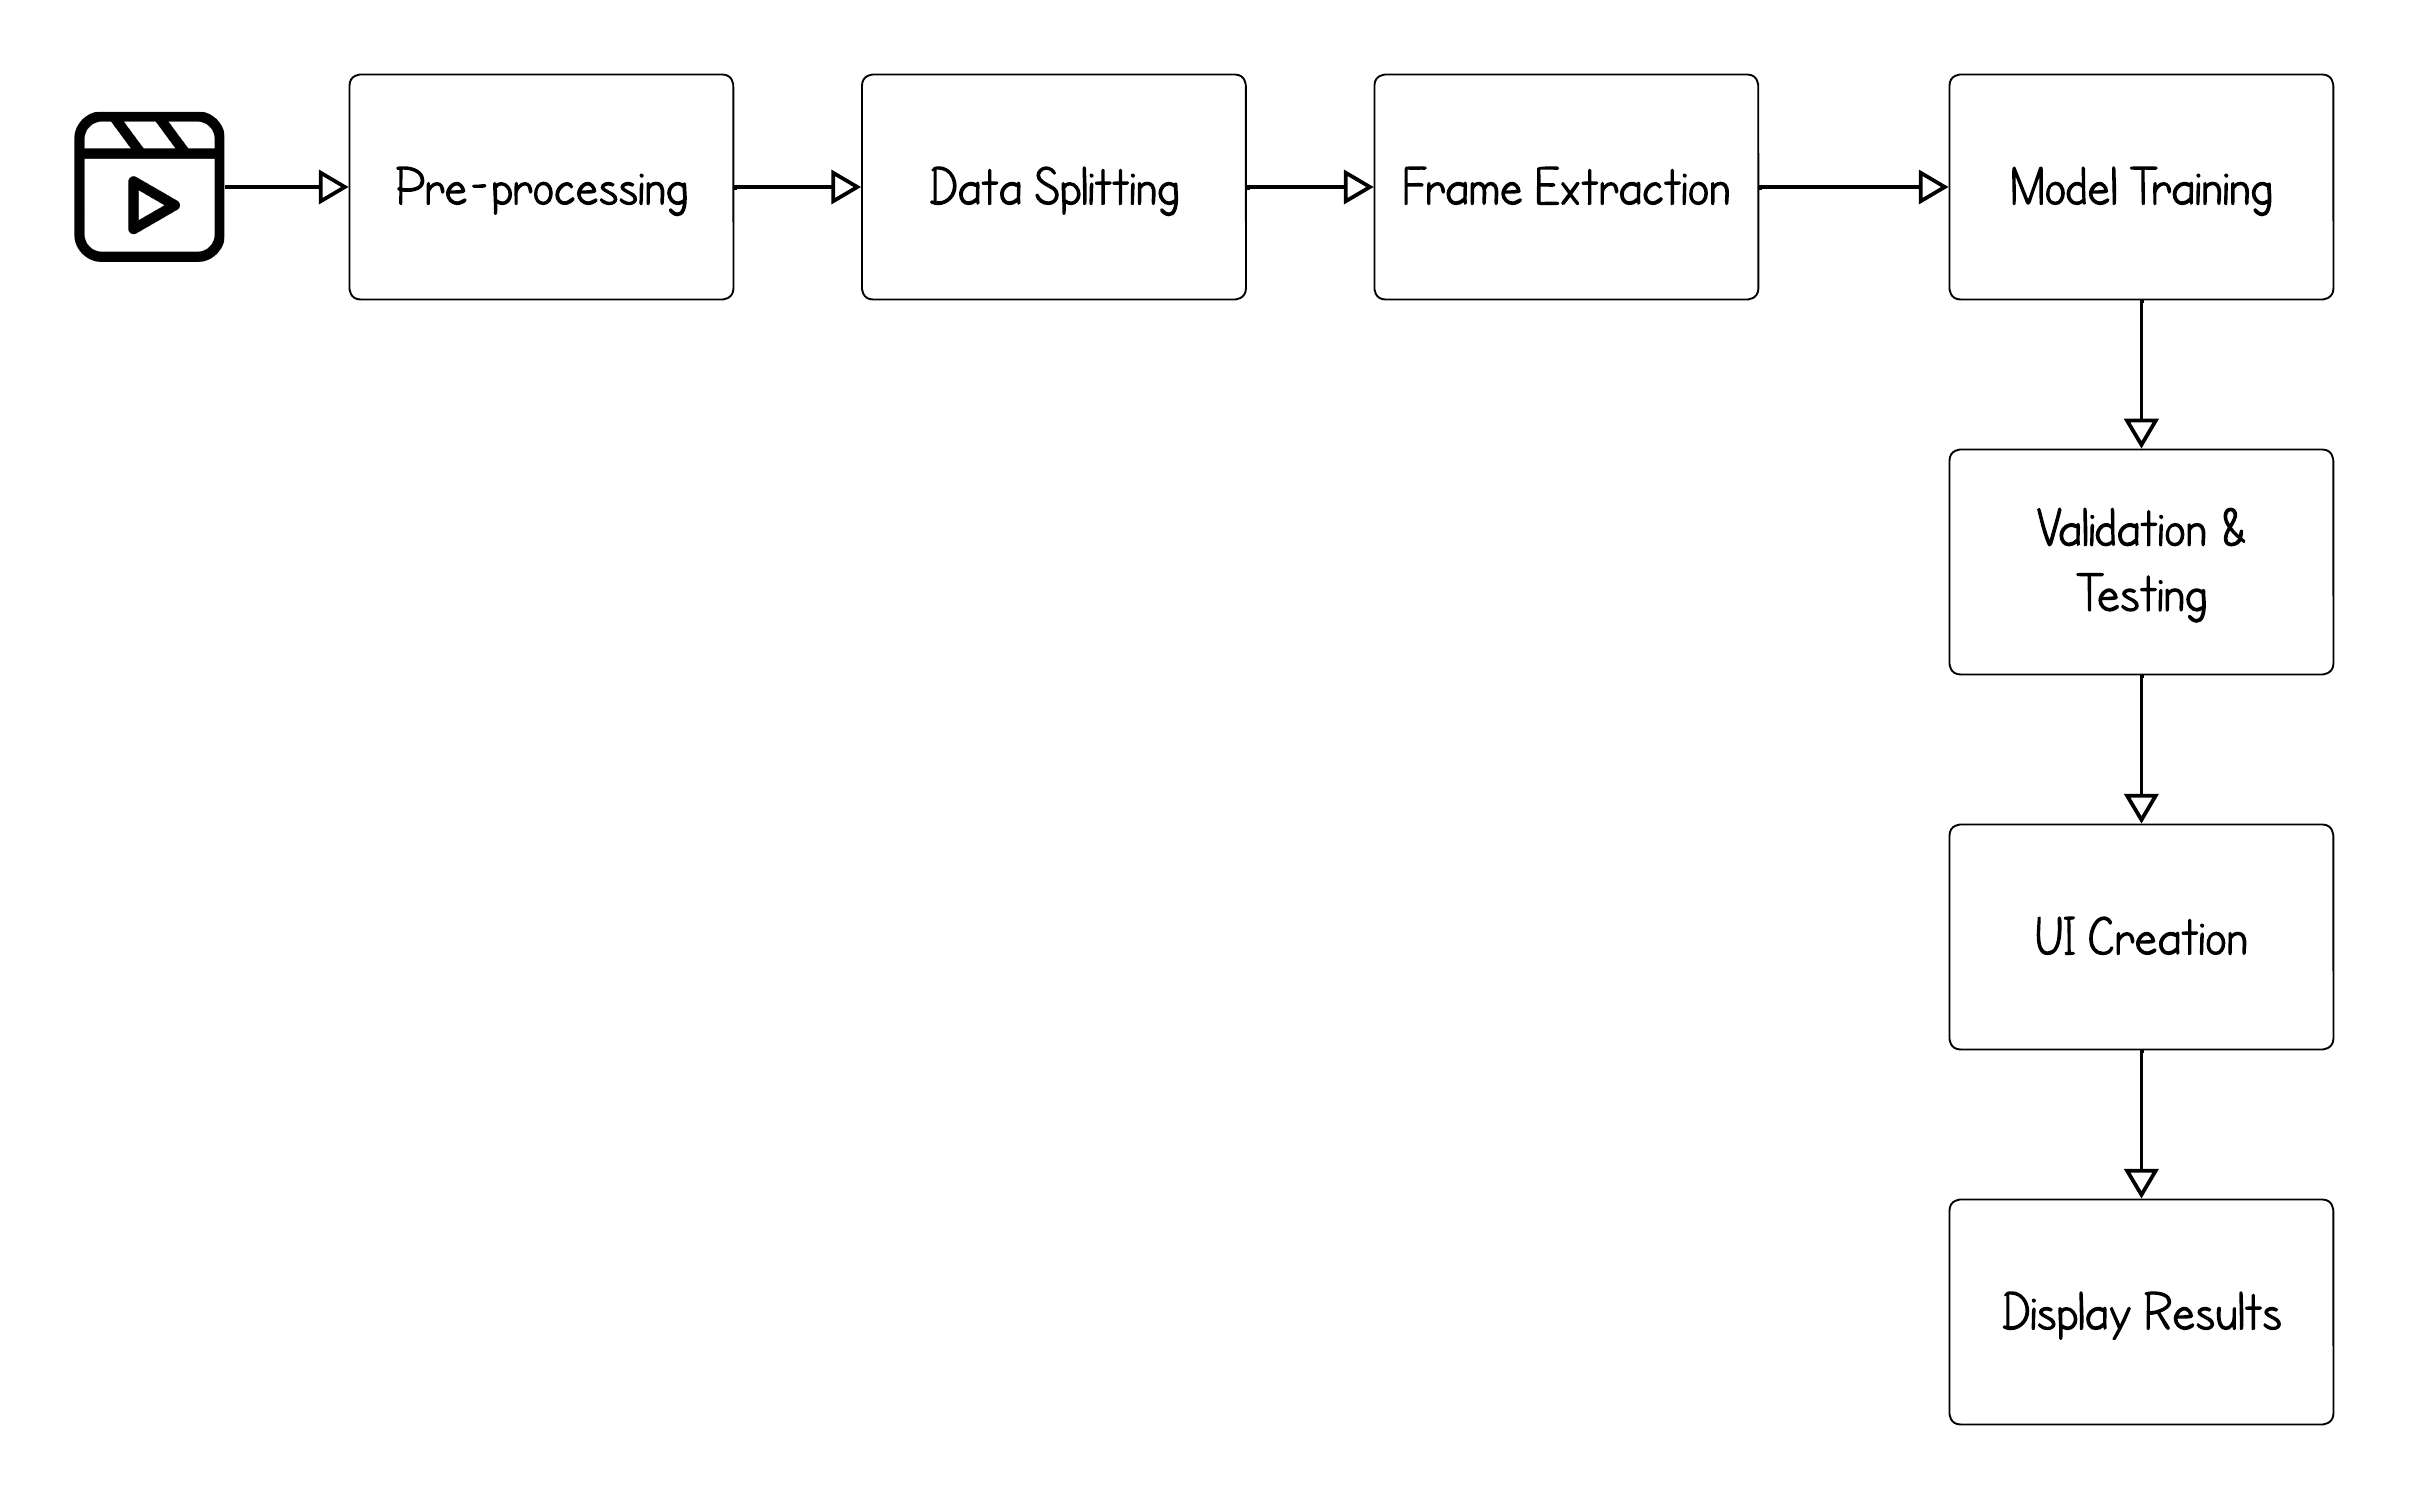
\includegraphics[width=1\linewidth]{img/Block_diagram.png}
    \caption{Block diagram of the system}
    \label{fig:Block Diagram of the system}
\end{figure}
	

\section{Description of working flow of proposed system}
\begin{enumerate}
  
    \item \textbf{\large Selection of Dataset:}

    
    Lipreading datasets (AVICar, AVLetters, AVLetters2, BBC TV, CUAVE, OuluVS1, OuluVS2) are plentiful \cite{zhou2014review}\cite{chung2017lip}, but most only contain single words or are too small. One exception is the \textbf{GRID corpus} (Cooke et al., 2006), which has audio and video recordings of 34 speakers who produced 1000 sentences each, for a total of 28 hours across 34000 sentences.

    We used the \textbf{GRID corpus} over other datasets because it is sentence-level and has the most data. The sentences are drawn from the following grammar: \textbf{\textit{command} + \textit{color} + \textit{preposition} + \textit{letter} + \textit{digit} + \textit{adverb}}. The categories consist of, respectively, \{bin, lay,place, set\}, \{blue, green, red, white\}, \{at, by, in, with\}, \{a, . . . , z\}\textbackslash\{w\}, \{zero, . . . , nine\}, and \{again, now, please, soon\}, yielding 64000 possible sentences.

    For example, two sentences in the data are \textbf{“set blue by A four please”} and \textbf{“place red at C zero again”}.\pagebreak
    \begin{figure}
  \centering
    \begin{subfigure}{0.4\textwidth}
    \centering
    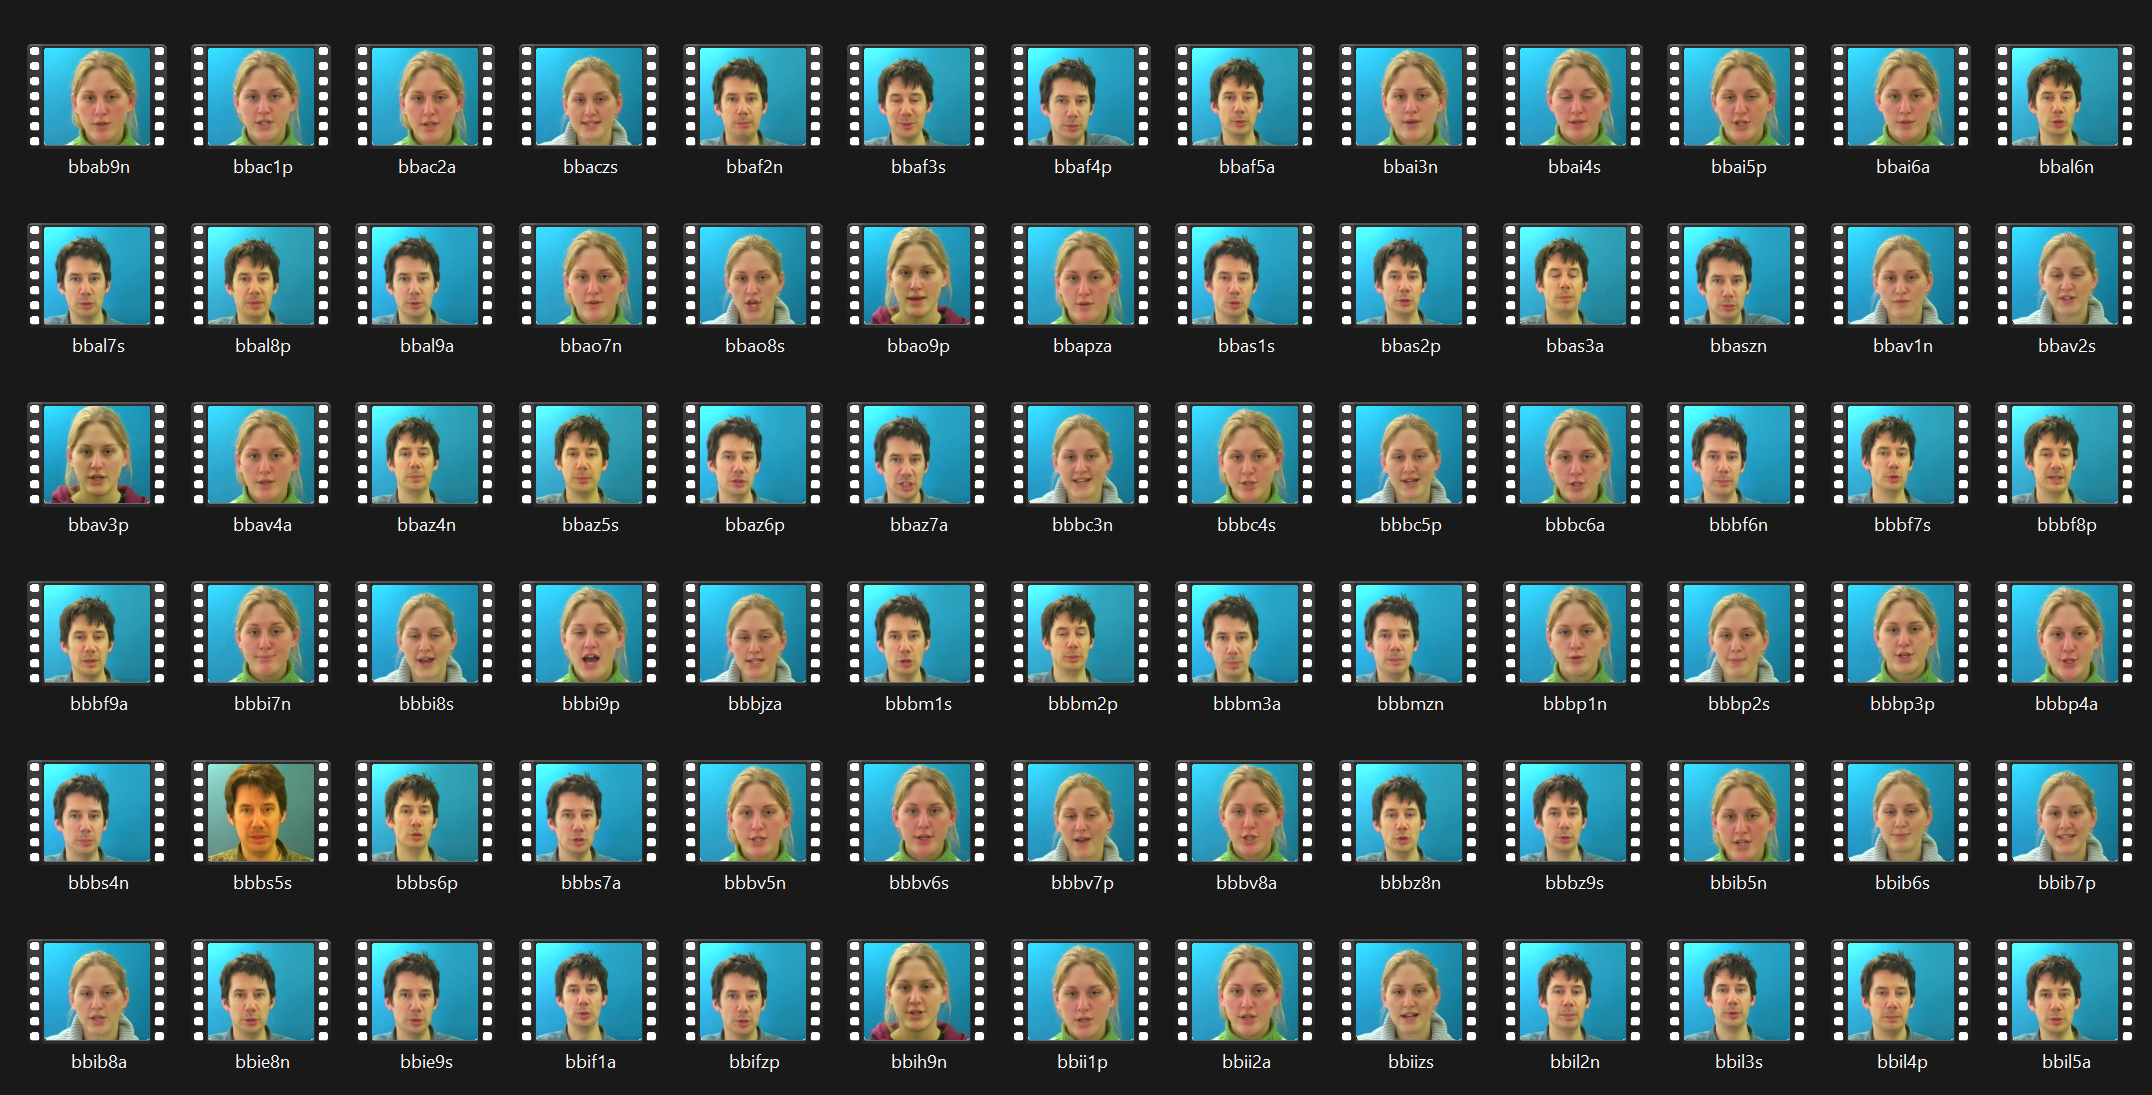
\includegraphics[width=1.60\linewidth]{img/Dataset_videos.png}
    \caption{Videos}
    \label{fig:sub1}
  \end{subfigure}%
  % \hspace{2em}% Adjust the horizontal space between the subfigures
  \begin{subfigure}{0.8\textwidth}
    \centering
    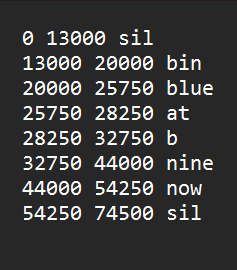
\includegraphics[width=0.3\linewidth]{img/alignments.png}
    \caption{Alignments of Videos}
    \label{fig:sub2}
  \end{subfigure}

  \caption{Grid Corpus dataset}
  \label{fig:main}
\end{figure}

\item \textbf{\large Dataset Pre-processing:}

In the selected Dataset \textbf{GRID corpus} there are total of 34 talkers(18 male,16 female),but to train our model we used only data of 1 male speaker and 1 female speaker which contains of about 1000 videos and 1000 alignments of each individual video. The data was split into different sets to use for training and validation.\textbf{80\%} of the data was provided to training set and \textbf{20\%} of the videos were provided into validation set. We used data from another male speaker for testing. 

\item \textbf{\large Feature Extraction:}
In our project, the region of interest lies within the lip and mouth area of the speaker. To segregate the region of interest from the whole image, the following slicing mechanism with static facial coordinates was used:
\begin{center}
    \texttt{frames.append(frame[190:236,85:260,:])}
\end{center}
 Here, the .append() method in Python is being used to store sliced video frames. Inside the method, there is a set of facial coordinates used to focus on the required part of the face.
 \begin{itemize}
     \item \textbf{190:236} : This selects rows 190 to 235 (inclusive). It specifies the vertical range of the region of interest.
     \item \textbf{80:280} : This selects columns 80 to 279 (inclusive). It specifies the horizontal range of the region of interest.
     \item \textbf{\large:} : This indicates that no specific color channels are selected and all of the RGB channels are to be used during slicing.
 \end{itemize}

 \begin{figure}
  \centering

  \begin{subfigure}{0.4\textwidth}
    \centering
    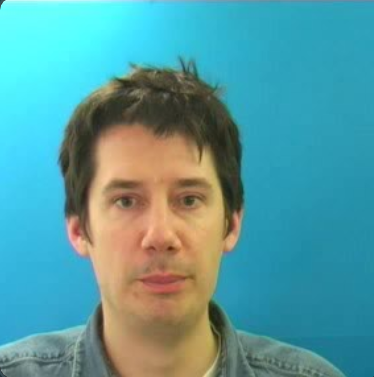
\includegraphics[width=0.9\linewidth]{img/face.png}
    \caption{Before Slicing}
    \label{fig:sub1}
  \end{subfigure}%
  \hspace{2em}% Adjust the horizontal space between the subfigures
  \begin{subfigure}{0.4\textwidth}
    \centering
    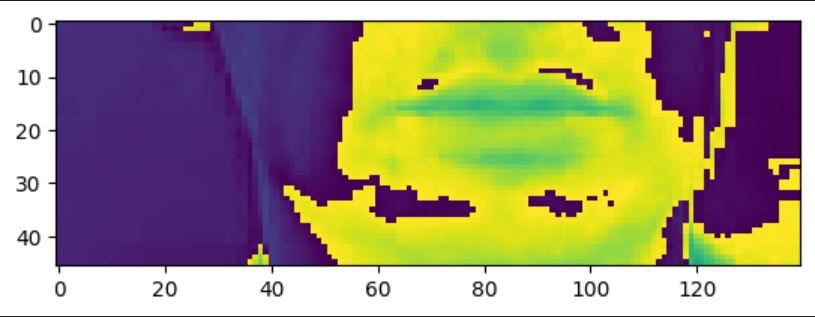
\includegraphics[width=1.2\linewidth]{img/cropped.png}
    \caption{After slicing}
    \label{fig:sub2}
  \end{subfigure}

  \caption{Feature Extraction}
  \label{fig:main}
\end{figure}

\newpage
\item \textbf{\large Model Training:}
\begin{itemize}
    \item \textbf{Convolution 3D layer:}\\
The Conv3D layers in the our model perform 3D convolution, extracting spatial features from input volumes. These layers use learnable filters to convolve across three dimensions, capturing complex patterns in video or volumetric data. The extracted features are crucial for tasks like video classification, action recognition, and medical imaging, enhancing model performance.

 \item \textbf{Max-Pooling3D:}\\
 Max pooling in the model reduces spatial dimensions by selecting the maximum values from neighboring groups in feature maps. Applied after 3D convolutional layers, it efficiently captures essential spatial information, aiding in feature extraction. This downsampling technique enhances the model's capacity for tasks such as video analysis and volumetric data processing.
 \item \textbf{Time-distributed layer:}\\
 In the model, the TimeDistributed layer processes the output of preceding layers independently at each time step. Applied after 3D convolutional and max-pooling layers, it facilitates the capture of temporal dependencies in sequential data, enhancing the model's ability for tasks like video analysis and spatiotemporal feature extraction.
 \item \textbf{Bi-Directional LSTM:}\\
 The Bidirectional LSTM layers in the model process sequential data bidirectionally, capturing dependencies in both forward and backward directions. These layers enhance temporal understanding, crucial for tasks like video analysis. With dropout regularization, they mitigate overfitting, improving generalization. The bidirectional nature enables the model to comprehend complex temporal relationships, making it suitable for applications requiring sequential data interpretation.\\
 \begin{figure}[h]
     \centering
     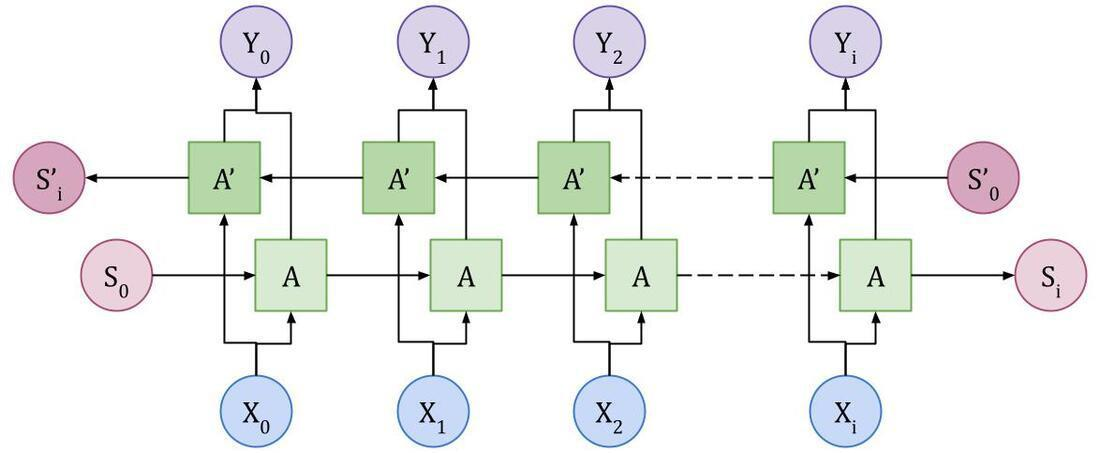
\includegraphics[width=1\linewidth]{img/BI-lstm.jpg}
     \caption{Bi-directional LSTM}
     
 \end{figure}

 Bidirectional Long Short-Term Memory (BI-LSTM) is an extension of the traditional Long Short-Term Memory (LSTM) architecture, commonly used in deep learning for sequential data processing, such as in natural language processing tasks or time series analysis. The mathematics behind BI-LSTM involves understanding the LSTM cell and how bidirectionality is incorporated.

\item \textbf{LSTM Cell:}\\
 \begin{enumerate}
 \item \textbf{Forget Gate:}
A sigmoid function is usually used for this gate to make the decision of what information needs to be removed from the LSTM memory. This decision is essentially made based on the value of \(h_{t-1}\) and \(x_t\). The output of this gate is \(f_t\), a value between 0 and 1, where 0 indicates completely getting rid of the learned value, and 1 implies preserving the whole value. This output is computed as:
\[ f_t = \sigma(W_{fh}h_{t-1} + W_{fx}x_t + b_f) \]
where \(b_f\) is a constant and is called the bias value.

 \item \textbf{Input Gate:}
 This gate makes the decision of whether or not the new information will be added into the LSTM memory. This gate consists of two layers: 1) a sigmoid layer, and 2) a "tanh" layer. The sigmoid layer decides which values need to be updated, and the tanh layer creates a vector of new candidate values that will be added into the LSTM memory. The outputs of these two layers are computed through:
\begin{align*}
    & i_t = \sigma(W_{ih}h_{t-1} + W_{ix}x_t + b_i) \\
    & \tilde{c}_t = \tanh(W_{ch}h_{t-1} + W_{cx}x_t + b_c)
\end{align*}
where \(i_t\) represents whether the value needs to be updated or not, and \(\tilde{c}_t\) indicates a vector of new candidate values that will be added into the LSTM memory. The combination of these two layers provides an update for the LSTM memory in which the current value is forgotten using the forget gate layer through multiplication of the old value (i.e., \(c_{t-1}\)) followed by adding the new candidate value \(i_t \cdot \tilde{c}_t\). The following equation represents its mathematical equation:
\[ c_t = f_t \cdot c_{t-1} + i_t \cdot \tilde{c}_t  \]
where \(f_t\) is the result of the forget gate, which is a value between 0 and 1 where 0 indicates completely getting rid of the value, whereas 1 implies completely preserving the value.


\item \textbf{Output Gate:}
This gate first uses a sigmoid layer to make the decision of what part of the LSTM memory contributes to the output. Then, it performs a non-linear tanh function to map the values between $-1$ and $1$. Finally, the result is multiplied by the output of a sigmoid layer. The following equations represent the formulas to compute the output:
\begin{align*}
    & o_t = \sigma(W_{oh}h_{t-1} + W_{ox}x_t + b_o) \\
    & h_t = o_t \cdot \tanh(c_t) 
\end{align*}
where \(o_t\) is the output value, and \(h_t\) is its representation as a value between $-1$ and $1$.\\

\item \textbf{Bidirectional Aspect:}\\
In a BI-LSTM, the sequence is processed in both forward and backward directions. The final hidden state (\(h_t\)) for a time step is the concatenation of the forward (\(h_t^{\text{forward}}\)) and backward (\(h_t^{\text{backward}}\)) hidden states.

\[ h_t = [h_t^{\text{forward}}, h_t^{\text{backward}}] \]

This bidirectional processing allows the model to capture information from both past and future contexts, enhancing its ability to understand sequential dependencies.

In summary, the mathematics behind BI-LSTM involves the computations within the LSTM cell, which includes forget gates, input gates, cell state updates, and output gates. The bidirectional aspect involves processing the sequence in both forward and backward directions to capture information from past and future contexts.








 \end{enumerate}
 \item \textbf{Drop-Out:}\\
 The Dropout layers in our model introduces regularization by randomly setting a fraction of input units to zero during training. This prevents overfitting, improving model generalization. Applied after Bidirectional LSTM layers, Dropout enhances the network's robustness and aids in better capturing temporal dependencies in sequential data.
 \item \textbf{Dense Layer:}\\
 The Dense layer is pivotal in our model, is fully connected, linking every neuron to the preceding layer's neurons. With 41 output units, it captures intricate patterns from the learned features, playing a key role in final predictions. Particularly impactful in multiclass classification, this layer contributes to the model's ability to discern and classify diverse patterns in the input data.
 
\end{itemize}



\item \textbf{\large Activation Function :}
\begin{enumerate}
    \item \textbf{Softmax}\\
         The softmax activation function is designed to work with multi-class classification tasks, where an input needs to be assigned to one of several classes.The softmax function uses a vector of real numbers as input and returns another vector of the same dimension, with values ranging between 0 and 1. Because these values add up to 1, they represent valid probabilities. The mathematical formula for the softmax function is given by:
         
        \begin{align*}
            \text{Softmax}(\mathbf{z})_i = \frac{e^{z_i}}{\sum_{j=1}^{K} e^{z_j}}
        \end{align*}

Where:

\text{Softmax}(\mathbf{z})$_i$ \text{ represents the $i$-th element of the resulting softmax vector.}


\mathrm{e} \text{ denotes Euler's number, the base of the natural logarithm.}\\

\(Z_i\)  is the \(i-th\) element of the input vector
The denominator \( \sum_{j=1}^{K} e^{z_j} \) represents the sum of the exponentiated values of all elements of \( \mathbf{z} \), ensuring that the resulting vector represents a valid probability distribution over the classes.

The softmax activation function is generally used for multi class classification in computer vision and natural language processing. In our project the goal is to classify the lip movement into corresponding phonemes or words. The softmax function is used in output layer of the neural network to provide a probability distribution over possible classes.Each class represents a different word or phoneme, and the class with the highest probability is chosen as the output. By using the softmax function in the output layer of the neural network, the lip reading system can effectively model the uncertainty in predicting spoken words or phonemes based on visual cues from lip movements. It provides a probabilistic interpretation of the predictions, which can be useful for downstream tasks such as language understanding or human-computer interaction.

\item \textbf{Rectified Linear Unit(Relu) function:}\\
The rectified linear activation function or ReLU is a non-linear function or piecewise linear function that will output the input directly if it is positive, otherwise, it will output zero.The Relu function can be mathematically defined by :
   \[ \text{ReLU}(x) = \max(0, x) \]

Where \textbf{x} is the input to the function.

 The ReLU function outputs the input value if it's greater than zero, otherwise, it outputs zero. Graphically, it looks like a linear function for $x\geq0$, with a slope of 1, and zero for x$<$0. The ReLU function is computationally efficient as it can be implemented by simply thresholding a matrix of activations at zero. It also helps mitigate the vanishing gradient problem, which is a difficulty encountered when training neural networks. In our lip reading project, Relu activation function are used in hidden layers.These hidden layers process the extracted features, transforming them through linear transformations followed by nonlinear activations. By using ReLU activation, the network can introduce nonlinearity, enabling it to learn complex patterns and relationships between the input features.
\end{enumerate}   

\item \textbf{\large Optimizer:}\\
We used the Adam optimizer, a popular optimization algorithm used in TensorFlow and other deep learning frameworks. It stands for Adaptive Moment Estimation and combines the advantages of two other popular optimization methods: RMSProp and Momentum. ADAM is a stochastic gradient descent algorithm based on estimation of 1st and 2nd-order moments. The algorithm estimates 1st-order moment (the gradient mean) and 2nd-order moment (element-wise squared gradient) of the gradient using exponential moving average, and corrects its bias. The final weight update is proportional to learning rate times 1st-order moment divided by the square root of 2nd-order moment. We used the ADAM optimizer in our source code by simply specifying it as our optimizer of choice.

\item \textbf{\large Testing \& Validation:}\\
A small subset of the GRID corpus dataset has been used as test data while validation is done alongside training by splitting the initial dataset as mentioned earlier.\\
Two metrics, \textbf{Word Error Rate(WER)} and \textbf{Character Error Rate(CER)} are used as performance evaluation parameters. WER(or CER) is defined as the minimum number of word (or character) insertions, substitutions, and deletions required to transform the prediction into the ground truth, divided by the number of words(or characters) in the ground truth. Note that WER is usually equal to classification error when the predicted sentence has the same number of words as the ground truth, particularly in our case since almost all errors are substitution errors.
For eg: Consider a random instance where our model predicts a ground truth of \textbf{"bin blue by m zero please"} as \textbf{"bin blue by b zero please"}.
In this case, the \textbf{WER} is calculated to be 0.1667 and the \textbf{CER} is 0.04.
\newpage
\item \textbf{\large Description of the model:}
\begin{table}[H]
\begin{tabularx}{\textwidth}{|l|X|X|}
    \hline
    \textbf{Layer Type} & \textbf{Output Shape} & \textbf{Summary} \\
    \hline
    Conv3D(activation='relu') & (None, 75, 46, 175, 128) & 3D convolutional layer for spatial feature extraction. \\
    \hline
    MaxPooling3D & (None, 75, 23, 87, 128) & Max pooling to reduce spatial dimensions. \\
    \hline
    Conv3D(activation='relu') & (None, 75, 23, 87, 256) & 3D convolutional layer for spatial feature extraction. \\
    \hline
    MaxPooling3D & (None, 75, 11, 43, 256) & Max pooling to reduce spatial dimensions. \\
    \hline
    Conv3D(activation='relu) & (None, 75, 11, 43, 75) & 3D convolutional layer for spatial feature extraction. \\
    \hline
    MaxPooling3D & (None, 75, 5, 21, 75) & Max pooling to reduce spatial dimensions. \\
    \hline
    TimeDistributed & (None, 75, 7875) & Applies the flatten operation to each time step. \\
    \hline
    Bidirectional(LSTM,activation='Tanh') & (None, 75, 256) & Bidirectional LSTM capturing temporal dependencies. \\
    \hline
    Dropout & (None, 75, 256) & Dropout for regularization. \\
    \hline
    Bidirectional(LSTM,activation='Tanh') & (None, 75, 256) & Bidirectional LSTM capturing temporal dependencies. \\
    \hline
    Dropout & (None, 75, 256) & Dropout for regularization. \\
    \hline
    Dense(activation='softmax') & (None, 75, 41) & Dense output layer with 41 units. \\
    \hline
\end{tabularx}
\caption{Description of Each Layer in the Model}
\end{table}
\newpage
\item \textbf{\large UI generation}

    To make the project user-friendly, a graphical interface has been developed using the Python library Streamlit. Within this interface, users can select videos from a dropdown menu. Upon selection, the chosen video is displayed in MP4 format. Additionally, a Mp4 of the video is shown at a slower pace, facilitating observation of lip movements.
    The machine learning model decodes lip movements into tokens, representing different words. These tokens are then displayed in the interface for users to observe how the model works.
    
    Finally, the interface presents both the original text spoken in the video and the text predicted by the model. 
    \begin{figure}[H]
        \centering
        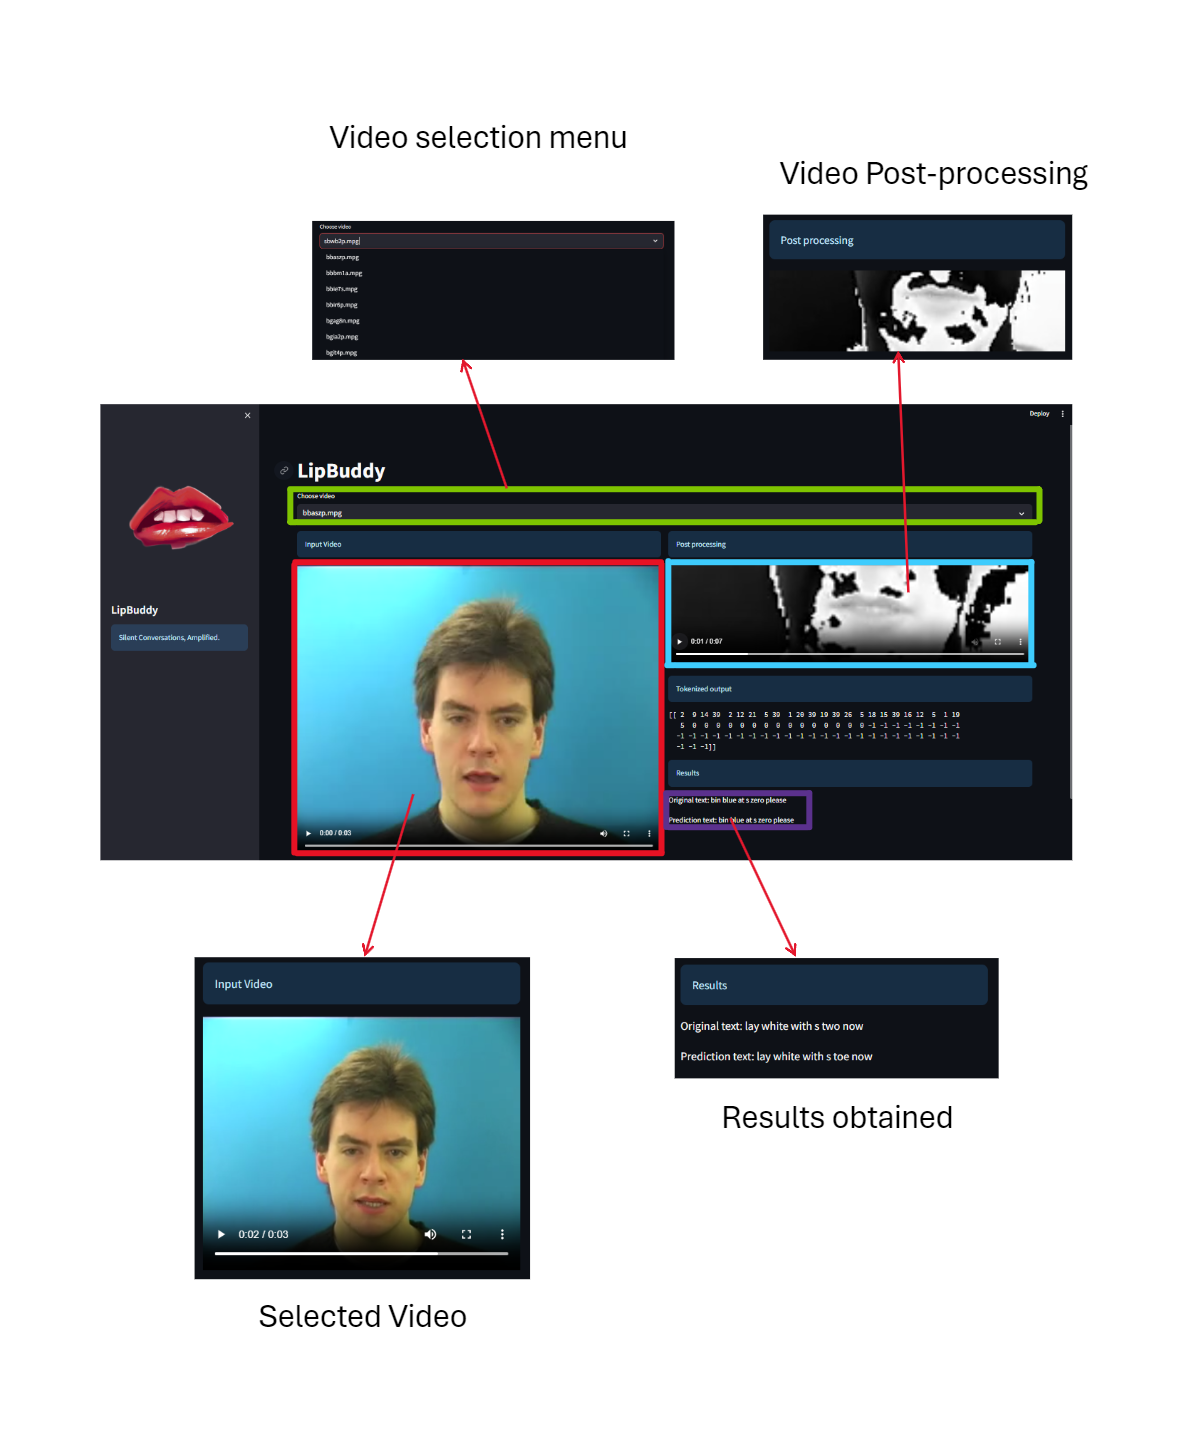
\includegraphics[width=1\linewidth]{img/null.png}
        \caption{UI of LipReading project}
        
    \end{figure}
\end{enumerate} 
    